% !TEX root = deckblatt3a.tex

\section{Invertierender Schmitt-Trigger}
\subsection{Simulationsschaltung}
\begin{figure}[H]
  \begin{center}
    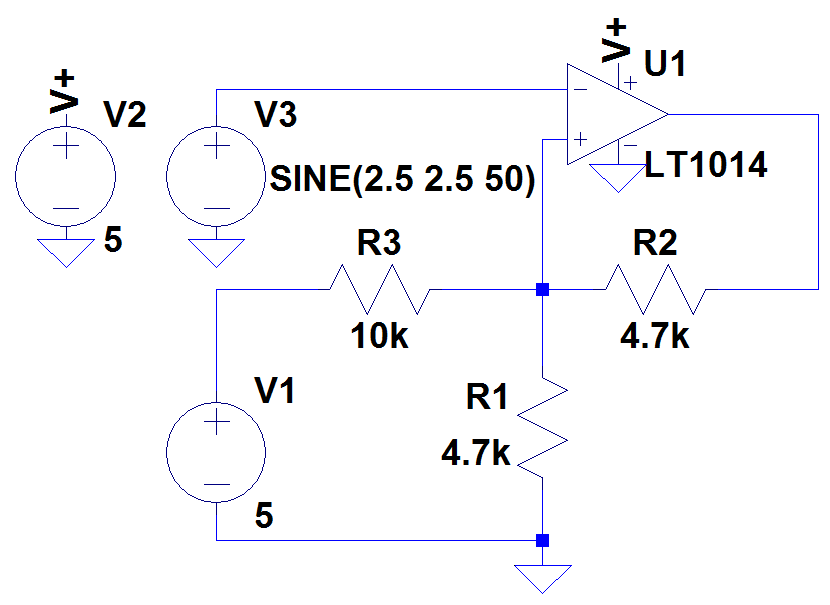
\includegraphics[width=1\textwidth]{./Schaltungen/InvertierenderSchmittTrigger.png}
    \caption{Simulationsschaltung}
  \end{center}
\end{figure}
\noindent
Da das Eingangsignal an den invertierenden Eingang geschaltet ist, ist diese OPV Schaltung auf jeden Fall invertierend. Die Ausgangsspannung wird auf den nicht-invertierenden Eingang r\"uckgekoppelt, das hei\ss{}t es handelt sich um eine Mittkopplung, das hei\ss{}t der OPV wird bei jedem Eingangssignal entweder nach oben oder nach unten \"ubersteuern.

\subsection{Berechnung Superpositionsprizip}
$U_{high}=4,39V$ \\
$U_{low}=0,029V$ \\ \\
$R_{12}=2,35k\Omega$ \\
$R_{13}=3,19k\Omega$ \\ \\
\begin{itemize}
  \item \textbf{1. Fall: $U_{high}$} \\ \\
        \textbf{Kurzgeschlossen: $U_a$ }\\
        $U_{p1} = U_{VCC}*\frac{R_{12}}{R_{12}+R_3} = 5V * \frac{2,35}{12,35} = 0,951V$ \\ \\
        \textbf{Kurzgeschlossen $U_{VCC}$}\\
        $U_{p2} = U_{VCC}*\frac{R_{13}}{R_{13}+R_2} = 4,39V * \frac{3,19}{7,90} = 1,777VV$ \\ \\
        $\Rightarrow U_p = U_{p1} + U_{p1} = 2,728V$

  \item \textbf{2. Fall: $U_{low}$} \\ \\
        \textbf{Kurzgeschlossen: $U_a$ }\\
        $U_{p1} = U_{VCC}*\frac{R_{12}}{R_{12}+R_3} = 5V * \frac{2,35}{12,35} = 0,951V$ \\ \\
        \textbf{Kurzgeschlossen $U_{VCC}$}\\
        $U_{p2} = U_{VCC}*\frac{R_{13}}{R_{13}+R_2} = 0,029V * \frac{3,19}{7,90} = 0,0117V$ \\ \\
        $\Rightarrow U_p = U_{p1} + U_{p1} = 0,963V$
\end{itemize}


\subsection{Simulationen}
\begin{figure}[H]
  \centering
  \begin{tikzpicture}
    \begin{axis}[width=15cm, height=10cm, xmin=0, xmax=100e-3, xlabel={t}, ylabel={$U[V]$},y tick label style={grid=major}]
      \addplot table[x=time, y=V(n001), mark=none] {csv_files/invSchmitt_time1.csv};
      \addplot table[x=time, y=V(n002), mark=none] {csv_files/invSchmitt_time1.csv};
      \addplot table[x=time, y=V(n003), mark=none] {csv_files/invSchmitt_time1.csv};
    \end{axis}
  \end{tikzpicture}
  \caption{Sinus, $V_{PP}=5V, f=50Hz$,}
\end{figure}
\noindent
In dieser Abbildung ist die Eingangsspannung(blau), die Ausgangsspannung(rot) und die Schaltung am nicht-invertierenden Eingang(braun) des OPVs zu sehen. Mit den drei Widerst\"anden und der Referenzspannung von $5V$ werden die Schaltschwellen eingestellt. Die obigen Berechnungen werden in diesem Diagramm best\"atigt da man die Schaltschwellen von $0,963V$ bzw. $2,729V$ sehr gut erkennen kann. \\
Erreicht der Sinus $2,729V$ auf der steigenden Flanke springt der Ausgnag auf $-U_v$ in diesem Fall Masse, und werden $0,963V$ auf der fallenden Flanke erreicht springt der Ausgang auf $+U_v$ in diesem Fall $5V$. Der Wert der positiven Versorgungsspannung wird nicht genau erreicht da es sich nicht um einen 'Rail-to-Rail' OPV handelt.

\begin{figure}[H]
  \centering
  \begin{tikzpicture}
    \begin{axis}[width=15cm, height=10cm, xmin=0, xmax=1e-6, xlabel={t}, ylabel={$U[V]$},y tick label style={grid=major}]
      \addplot table[x=time, y=V(n001), mark=none] {csv_files/invSchmitt_time2.csv};
      \addplot table[x=time, y=V(n002), mark=none] {csv_files/invSchmitt_time2.csv};
      \addplot table[x=time, y=V(n003), mark=none] {csv_files/invSchmitt_time2.csv};
    \end{axis}
  \end{tikzpicture}
  \caption{Dreieck, $V_{PP}=5V, f=5MHz$}
\end{figure}
\noindent
Auf Grund der hohen Frequenz ben\"otigt die Innenbeschaltung des OPVs einige Zeit bis sich das System einschwingt. Danach ist ein Schmitt-Triggerverhalten zu erkennen, jedoch wird aufgrund des Tiefpassverhaltens sehr stark ged\"ampft.
